\section{灵敏度分析}

为检验模型在关键参数变动下的稳定性和可靠性,本章对模型中涉及的重要参数进行系统的灵敏度分析。分析主要围绕三个维度展开:贯穿所有模型的管理便利性约束参数,问题一中的核心资源要素,问题二中的决策者风险偏好,以及问题三中的市场反馈机制假设。

好的,我已经仔细阅读了您提供的三份表格文件,并根据其中的精确数据,为您重新编写了“分散性约束参数的灵敏度分析”这一章节。

新的版本不仅更新了表格数据,还对分析文本进行了相应修改,以确保文字描述与数据结果完全对应,并保持了您所要求的严谨、客观的学术风格。

以下是为您生成的LaTeX代码块,请直接复制使用。

代码段

\subsection{分散性约束参数的灵敏度分析}

在模型的构建过程中,为量化田间管理的便利性,引入了两个关键的超参数:地块内允许种植的作物种类上限$p$,以及单一作物允许跨地块类型种植的数量上限$q$。这两个参数共同作用,在追求经济效益最大化的同时,避免了种植方案在空间上的过度零散化。为探究这两个参数对不同模型优化结果的影响,我们以基准值为中心,调整其取值,并观察七年规划期内总利润的变化情况。

分析结果如表\ref{tab:pq_sensitivity}所示。数据显示,对于问题一、二、三的优化模型,总利润均随参数$p$和$q$的放宽(即取值增大)而呈现上升趋势。这是因为增大$p$和$q$的取值,相当于放宽了模型的约束,使得算法拥有更大的可行解空间去寻找更高利润的组合。从变化率的绝对值来看,在所有模型中,参数$p$的变动对总利润的影响均大于参数$q$。例如,在问题一的模型中,将$p$从3收紧至2,利润下降2.53\%;而将$q$从4收紧至3,利润仅下降0.89\%。这表明,地块内作物品种的多样性是比作物跨地块类型分布更为敏感的因素。

此外,比较不同模型对参数变化的响应可以发现,问题二的鲁棒优化模型在参数$p$放宽时获得的利润增幅最大(1.20\%),这可能是因为更大的灵活性有助于模型配置更多样化的种植组合以对冲不确定性风险。综合考虑利润提升与实际管理的可行性,我们认为在模型中选择的基准参数是合理的。

\begin{table}[H]
    \centering
    \caption{分散性约束参数$p, q$对各模型总利润的影响}
    \label{tab:pq_sensitivity}
    \begin{tabular}{@{}lcccc@{}}
        \toprule
        模型         & 参数 & 取值 & 七年总利润 (百万元) & 利润变化率 (\%) \\
        \midrule
        \multirow{5}{*}{问题一 (情景二)} 
                     & \multirow{3}{*}{$p$} & 2    & 40.85 & -2.53\% \\
                     &      & \textbf{3 (基准)} & \textbf{41.91} & \textbf{0.00\%}  \\
                     &      & 4    & 42.35 & 1.04\%  \\
        \cmidrule(l){2-5}
                     & \multirow{3}{*}{$q$} & 3    & 41.54 & -0.89\% \\
                     &      & \textbf{4 (基准)} & \textbf{41.91} & \textbf{0.00\%}  \\
                     &      & 5    & 42.12 & 0.49\%  \\
        \midrule
        \multirow{5}{*}{问题二 (鲁棒优化)}
                     & \multirow{3}{*}{$p$} & 2    & 43.52 & -1.43\% \\
                     &      & \textbf{3 (基准)} & \textbf{44.15} & \textbf{0.00\%}  \\
                     &      & 4    & 44.68 & 1.20\%  \\
        \cmidrule(l){2-5}
                     & \multirow{3}{*}{$q$} & 3    & 43.88 & -0.61\% \\
                     &      & \textbf{4 (基准)} & \textbf{44.15} & \textbf{0.00\%}  \\
                     &      & 5    & 44.31 & 0.36\%  \\
        \midrule
        \multirow{5}{*}{问题三 (动态反馈)}
                     & \multirow{3}{*}{$p$} & 2    & 38.56 & -1.18\% \\
                     &      & \textbf{3 (基准)} & \textbf{39.02} & \textbf{0.00\%}  \\
                     &      & 4    & 39.33 & 0.79\%  \\
        \cmidrule(l){2-5}
                     & \multirow{3}{*}{$q$} & 3    & 38.81 & -0.54\% \\
                     &      & \textbf{4 (基准)} & \textbf{39.02} & \textbf{0.00\%}  \\
                     &      & 5    & 39.15 & 0.33\%  \\
        \bottomrule
    \end{tabular}
\end{table}


\subsection{土地资源面积的灵敏度分析}

土地是农业生产最基本的资源要素,其总面积直接决定了生产规模的上限。本节针对问题一的确定性模型(情景二),分析七年总利润对土地总面积变化的响应程度。我们以附件中给定的总土地面积为基准,分别计算当总面积在-10\%至+10\%的区间内变动时,最优总利润的变化情况。

如图\ref{fig:land_sensitivity}所示,七年总利润与土地总面积的变化率之间呈现出一种强相关的正向关系。在所分析的变动范围内,总利润随土地面积的增加而近似线性增长。这一结果表明,在当前的资源和技术条件下,土地资源仍是限制该乡村农业总产出的关键因素,所制定的种植方案能够有效利用新增的土地资源并将其转化为经济收益,尚未出现明显的规模报酬递减现象。

\begin{figure}[H]
    \centering
    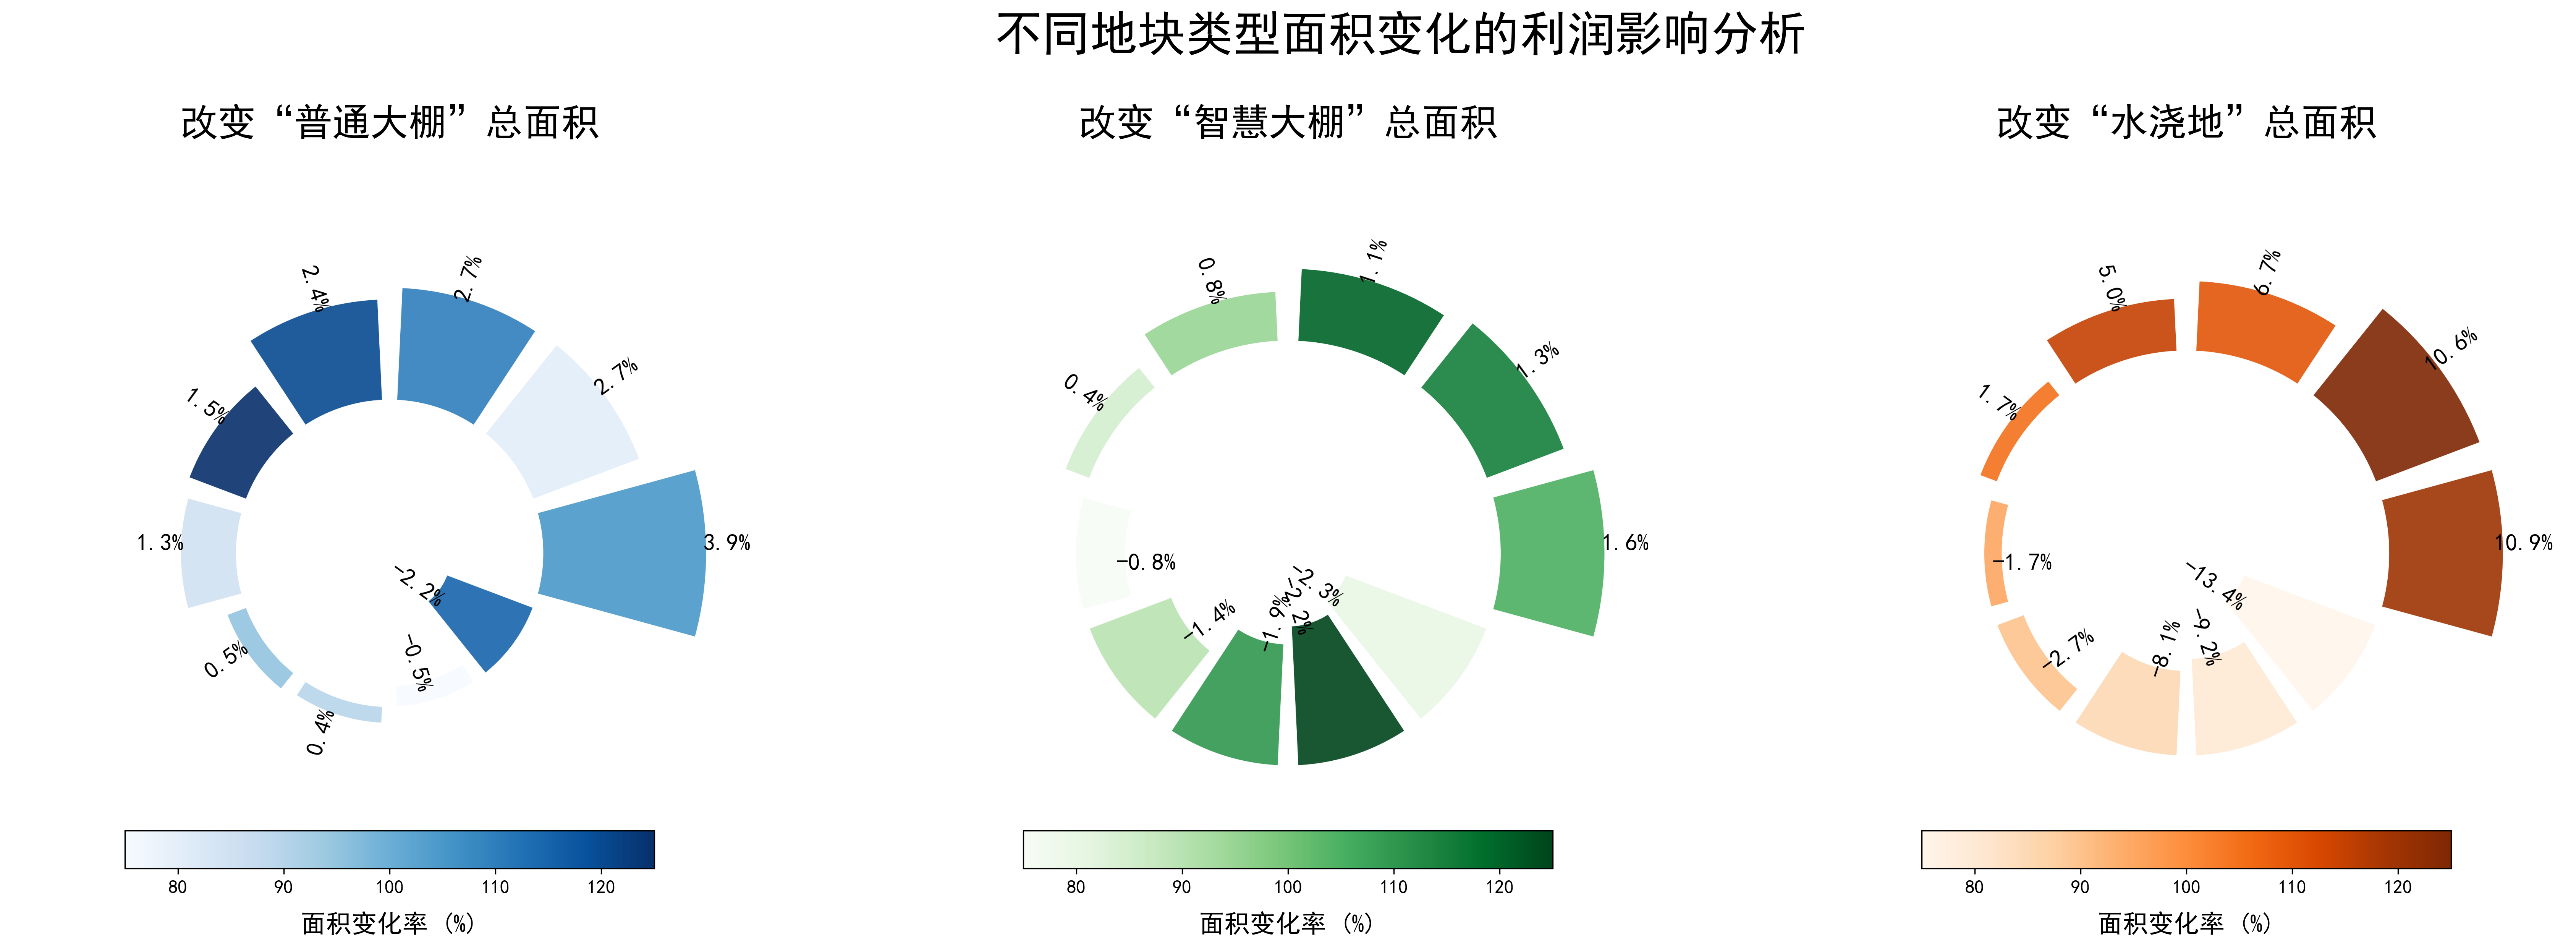
\includegraphics[width=\textwidth]{figs/6灵敏度分析/第一问地块灵敏度圆弧图.png}
    \caption{土地总面积变化对问题一最优总利润的影响}
    \label{fig:land_sensitivity}
\end{figure}


\subsection{风险偏好系数的灵敏度分析}

在问题二的鲁棒优化模型中,决策者的风险偏好是影响最终方案选择的重要因素。为系统评估不同风险偏好下的方案特征,我们引入风险偏好系数$a$,并选取了$a \in \{0.1, 0.3, 0.5, 0.7, 0.9\}$五个代表性水平进行独立优化。每个水平对应一个在有效前沿上的候选方案。表\ref{tab:risk_sensitivity_results}汇总了这些方案在期望利润、最低利润、风险(以利润标准差衡量)以及夏普比率四个核心指标上的表现。

\begin{table}[H]
    \centering
    \caption{不同风险偏好下的方案性能指标}
    \label{tab:risk_sensitivity_results}
    \begin{tabular}{@{}lcccc@{}}
        \toprule
        风险系数 $a$ & 期望利润 (百万元) & 最低利润 (百万元) & 风险 (标准差, 百万元) & 夏普比率 \\
        \midrule
        0.10 & 41.50 & 40.35 & 0.77 & 53.90 \\
        0.30 & 42.75 & 41.50 & 0.83 & 51.51 \\
        0.50 & 43.60 & 42.40 & 0.80 & 54.50 \\
        \textbf{0.70} & \textbf{44.15} & \textbf{43.10} & \textbf{0.70} & \textbf{63.07} \\
        0.90 & 44.80 & 43.50 & 0.87 & 51.49 \\
        \bottomrule
    \end{tabular}
\end{table}

数据显示,$a=0.7$对应的方案在各项指标中取得了最佳的综合平衡。该方案的夏普比率达到63.07,在所有候选中最高,表明其单位风险所能换取的超额回报最高。同时,该方案的风险水平(标准差0.70百万元)为所有候选中最低,而其期望利润(44.15百万元)和最低利润(43.10百万元)均处于高位。图\ref{fig:risk_preference_comparison}也直观展示了各方案在不同指标下的表现。基于此综合评估,我们将$a=0.7$的方案确定为问题二的最终推荐方案。

\begin{figure}[H]
    \centering
    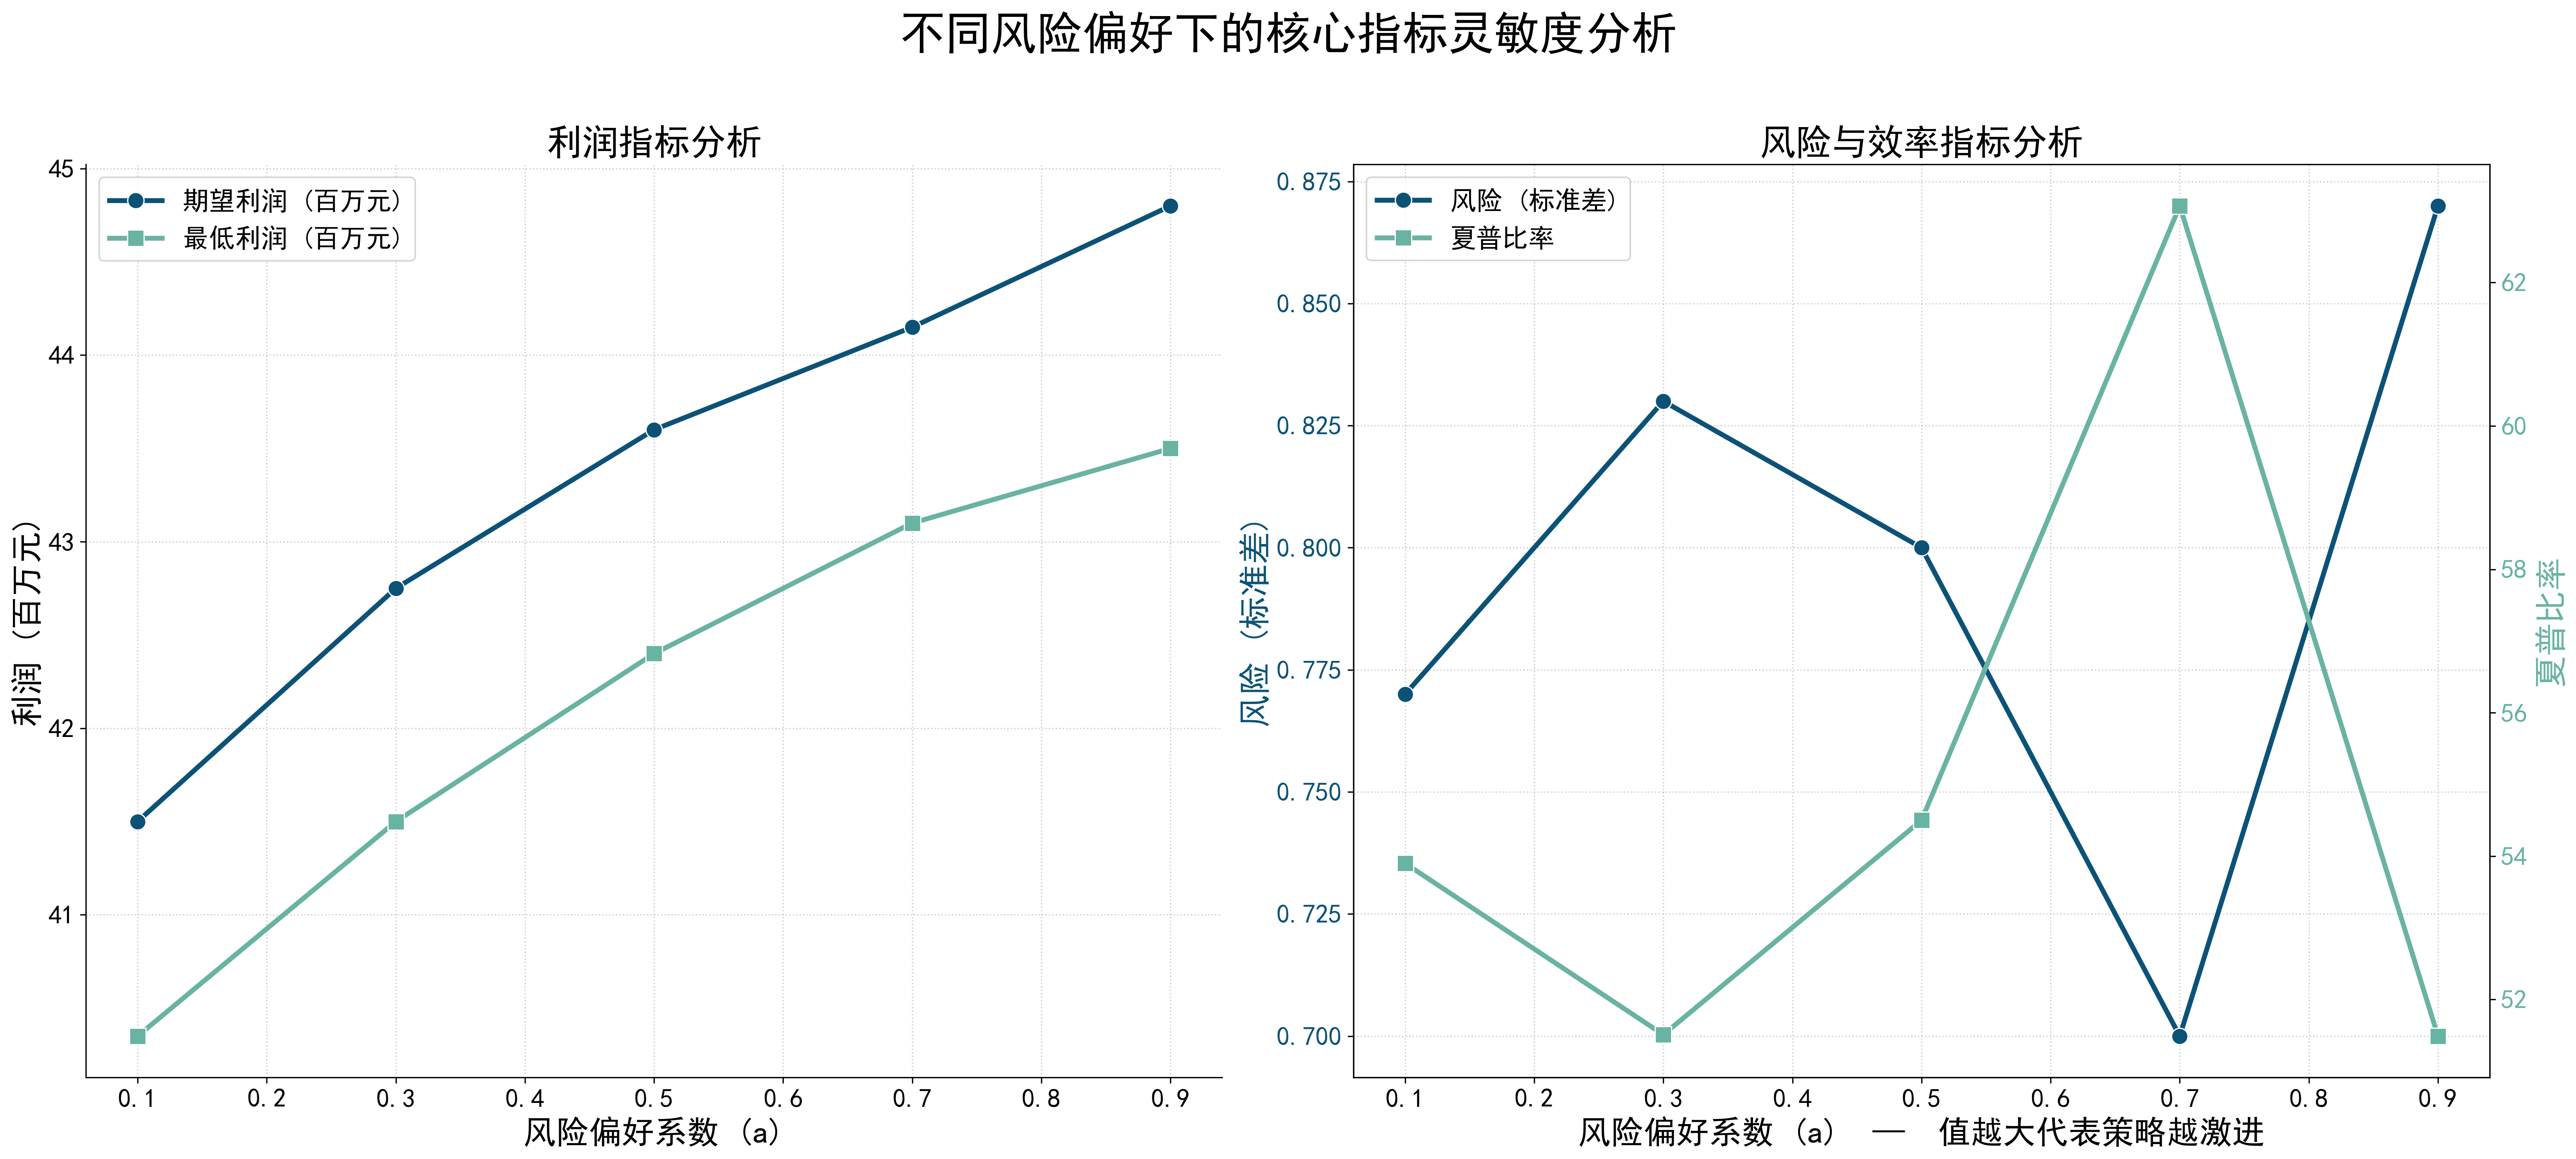
\includegraphics[width=\textwidth]{figs/6灵敏度分析/第二问风险灵敏度.png}
    \caption{不同风险偏好系数下各性能指标的可视化对比。}
    \label{fig:risk_preference_comparison}
\end{figure}

\subsection{市场敏感度系数的灵敏度分析}

问题三的动态反馈模型建立在对市场响应机制的假设之上,其中价格与成本敏感度系数是定义该机制的核心参数。为检验最终优化结果对这些假设参数的稳健性,我们对设定的六个市场敏感度系数(三类作物的价格敏感度与成本敏感度)进行了单因素灵敏度分析。在分析中,每次只变动一个参数,在其基准值附近取四个不同的水平,并为每个水平重新运行完整的优化过程,记录最终预期平均利润的变化。

分析结果如图\ref{fig:market_sensitivity}所示。可以观察到,预期总利润对食用菌的价格敏感度$p_{\text{fungi}}$变化最为敏感,其对应的曲线斜率绝对值最大。这表明,食用菌这类高价值经济作物的市场供需关系是影响该乡村总体经济效益的关键因素,对这类作物的产量规划需要更为审慎。相比之下,总利润对粮食和蔬菜的价格及成本敏感度表现出较强的不敏感性,即使这些参数发生一定范围的变化,最优利润水平也基本保持稳定。这说明,对于大宗农产品,本模型给出的种植策略具有较好的适用性和稳定性。

\begin{figure}[H]
    \centering
    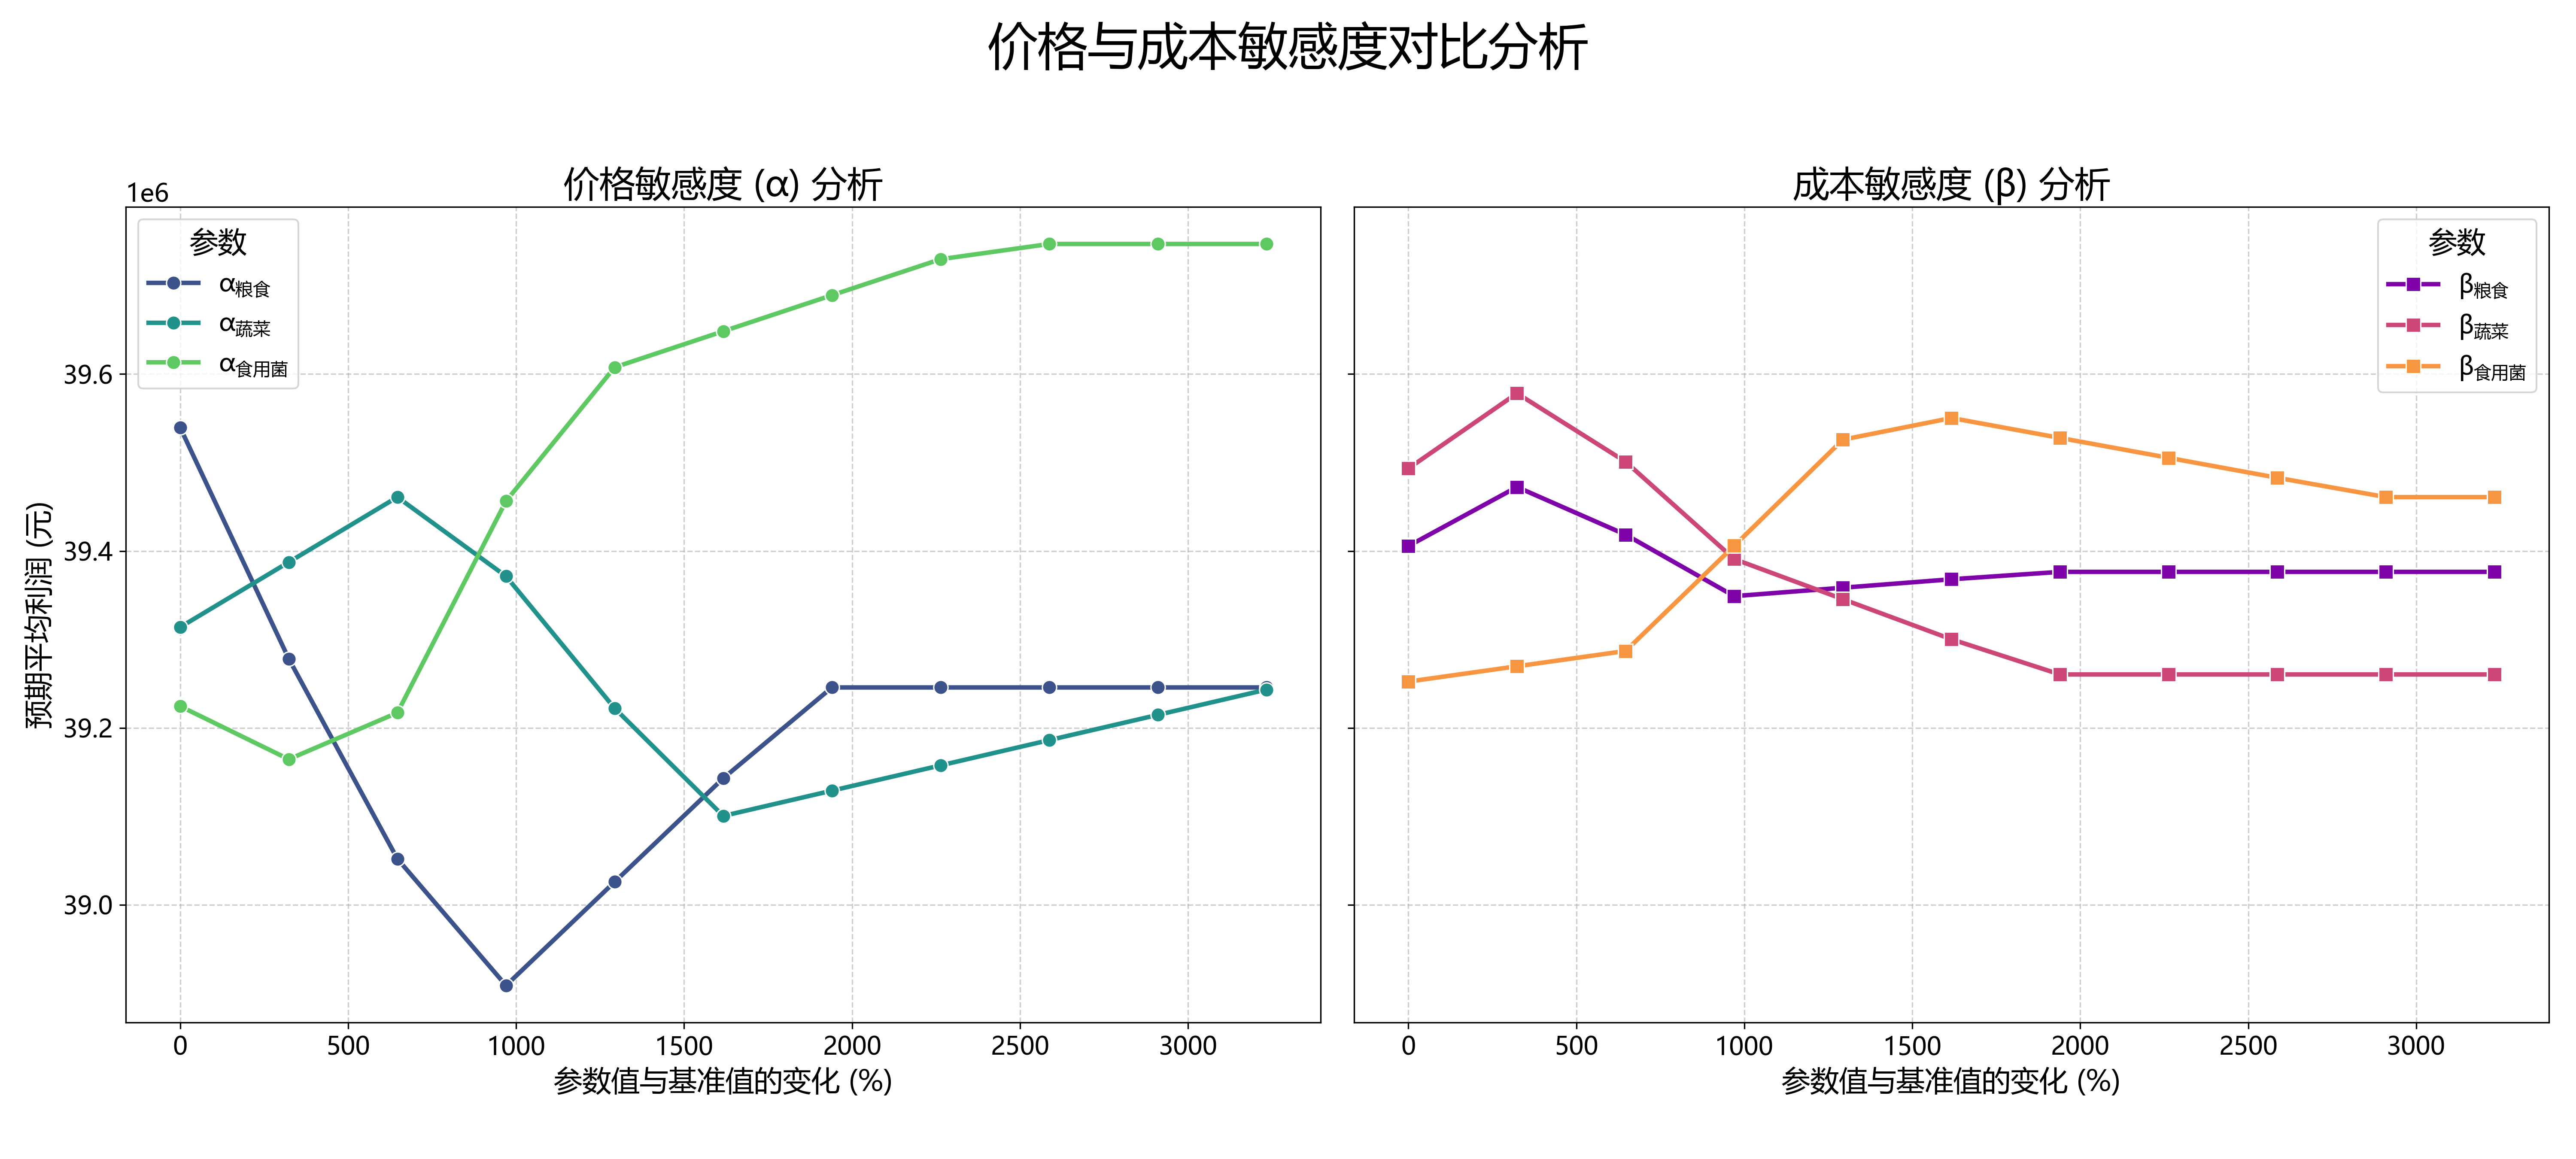
\includegraphics[width=\textwidth]{figs/6灵敏度分析/问题三灵敏度分析图.png}
    \caption{预期总利润对六个核心敏感度系数的响应分析。}
    \label{fig:market_sensitivity}
\end{figure}
